% Template LaTeX untuk Ujian Kualifikasi
% Program Studi Doktor Informatika
% Universitas Telkom

% Document Class
\documentclass[12pt,a4paper]{article}

% Packages
\usepackage[utf8]{inputenc}
\usepackage[T1]{fontenc}
\usepackage{mathptmx} % Times New Roman
\usepackage{courier}  % Courier for monospace
\usepackage{helvet}   % Helvetica for sans-serif
\usepackage{amsmath}
\usepackage[english,indonesian]{babel}
\usepackage{geometry}
\usepackage{setspace}
\usepackage{titlesec}
\usepackage{graphicx}
\usepackage{hyperref}
\usepackage{booktabs}
\usepackage{array}
\usepackage[format=hang,font=footnotesize,labelfont=bf]{caption}
\usepackage{enumitem}
\usepackage{parskip}
\usepackage{fancyhdr}
\usepackage{tocloft}
\usepackage{tabularx}
\usepackage{longtable}
\usepackage{ragged2e}  % For better text justification in bibliography

% Page Setup
\geometry{
    top=3cm,
    bottom=3cm,
    left=4cm,
    right=3cm
}

% Title Formatting
\titleformat{\section}
    {\normalfont\fontsize{16}{19}\bfseries\centering}{\thesection}{1em}{}
    
\titleformat{\subsection}
    {\normalfont\fontsize{12}{14}\bfseries}{\thesubsection}{1em}{}

\titleformat{\subsubsection}
    {\normalfont\fontsize{12}{14}\normalfont}{\thesubsubsection}{1em}{}

% Spacing
\onehalfspacing

% Header/Footer
\pagestyle{fancy}
\fancyhf{}
\fancyfoot[C]{\thepage}
\renewcommand{\headrulewidth}{0pt}

% Hyperref setup
\hypersetup{
    colorlinks=true,
    linkcolor=black,
    citecolor=black,
    filecolor=black,
    urlcolor=black,
}

% Table of Contents customization
\renewcommand{\contentsname}{DAFTAR ISI}
\renewcommand{\cfttoctitlefont}{\hfill\fontsize{16}{19}\selectfont\bfseries}
\renewcommand{\cftaftertoctitle}{\hfill}

% List of Tables customization
\renewcommand{\listtablename}{DAFTAR TABEL}
\renewcommand{\cftlottitlefont}{\hfill\fontsize{16}{19}\selectfont\bfseries}
\renewcommand{\cftafterlottitle}{\hfill}

% List of Figures customization
\renewcommand{\listfigurename}{DAFTAR GAMBAR}
\renewcommand{\cftloftitlefont}{\hfill\fontsize{16}{19}\selectfont\bfseries}
\renewcommand{\cftafterloftitle}{\hfill}

% List of Equations setup
\newcommand{\listequationsname}{DAFTAR RUMUS}
\newlistof{myequations}{equ}{\listequationsname}
\newcommand{\myequations}[1]{%
\addcontentsline{equ}{myequations}{\protect\numberline{\theequation}#1}\par}
\renewcommand{\cftequtitlefont}{\hfill\fontsize{16}{19}\selectfont\bfseries}
\renewcommand{\cftafterequtitle}{\hfill}
\setlength{\cftmyequationsindent}{0pt}

% Redefine \listofequations to use the custom list
\newcommand{\listofequations}{\listofmyequations}

% Subsection numbering format
\renewcommand{\thesubsection}{\arabic{section}.\arabic{subsection}}

% Custom Commands
\newcommand{\myTitle}[1]{\def\@myTitle{#1}}
\newcommand{\myName}[1]{\def\@myName{#1}}
\newcommand{\myNIM}[1]{\def\@myNIM{#1}}
\newcommand{\myYear}[1]{\def\@myYear{#1}}

% Redefine title
\makeatletter
% Initialize default values
\def\@myTitle{Implementasi Sistem Informasi}
\def\@myNIM{303012510004}
\def\@myName{Rolly Maulana Awangga}
\def\@myYear{Tahun}

\renewcommand{\maketitle}{
    \begin{titlepage}
        \centering
        \vspace*{0.5cm}
        
        % Judul Penelitian (bagian atas)
        {\fontsize{16}{20}\selectfont
        \textbf{Implementasi Sistem Informasi}\par}
        
        \vspace{1.5cm}
        
        % Tahap Ujian Kualifikasi
        {\fontsize{12}{14}\selectfont
        \textbf{Proyek / Internship}\par}
        
        \vspace{1.5cm}
        
        % NIM dan Nama
        {\fontsize{12}{14}\selectfont
        \textbf{\@myNIM}\par
        \textbf{\@myName}\par}
        
        \vspace{1.5cm}
        \vspace{1.5cm}
        \vspace{1.5cm}
     
        
        % Logo
        \IfFileExists{logo.png}{
            \includegraphics[width=0.5\textwidth]{logo.png}
        }{
            {\fontsize{16}{19}\bfseries Logo\par}
        }
        
        \vfill
        
        % Program Studi dan Informasi
        {\fontsize{16}{19}\selectfont
        \textbf{Program Studi Sarjana Terapan Teknik Informatika}\par
        \textbf{Sekolah Teknologi Informasi}\par
        \textbf{Universitas Logistik dan Bisnis Internasional}\par
        \textbf{Bandung}\par
        \textbf{2026}\par}
        
    \end{titlepage}
    \newpage
}
\makeatother

% SOTA Table Environment
\newenvironment{sototable}
    {\begin{table}[htbp]
    \centering
    \caption{State-of-the-Art Penelitian}
    \label{tab:sota}}
    {\end{table}}

% Word Count Environments
\newenvironment{summary}
    {}
    {}

\newenvironment{background}
    {}
    {}

\newenvironment{literaturereview}
    {}
    {}

\newenvironment{researchgap}
    {}
    {}

\newenvironment{novelty}
    {}
    {}

% Bibliography Style - APA-like with BibTeX
\usepackage[
    backend=bibtex,   % Menggunakan BibTeX (biber tidak berfungsi di sistem ini)
    style=authoryear, % Author-year citation style (APA-like)
    sorting=nyt,      % Sort by name, year, title
    maxbibnames=99,   % Tampilkan semua nama penulis
    dashed=false,     % Jangan gunakan dash untuk author yang sama
    url=false,        % Jangan tampilkan URL
    doi=true,         % Tampilkan DOI
]{biblatex}

\urlstyle{same} % Samakan font URL/DOI dengan teks utama

\addbibresource{references.bib}
\addbibresource{include.bib}
%\addbibresource{visualdecoding.bib} % Uncomment jika ingin menggunakan file bib tambahan

% Make \cite behave like \parencite (with parentheses)
\let\cite\parencite

% Custom citation formatting
\renewcommand*{\finalnamedelim}{\addspace\&\addspace}  % Ubah "and" jadi "&"
\renewcommand*{\nameyeardelim}{\addcomma\space}        % Tambahkan koma setelah author

% Remove "In:" from bibliography
\renewbibmacro{in:}{}

% Ensure pages are not bold
\DeclareFieldFormat{pages}{\normalfont #1}

% Custom format untuk memastikan ada spasi setelah "in"
\DeclareFieldFormat{booktitle}{\addspace\textit{#1}}
\DeclareFieldFormat{journaltitle}{\addspace\textit{#1}}

% Fix URL breaking untuk mencegah overflow
\setcounter{biburllcpenalty}{7000}
\setcounter{biburlucpenalty}{8000}

% Set bibliography to use ragged right alignment untuk mencegah overfull
\emergencystretch=1em
\appto{\bibsetup}{\sloppy\RaggedRight}



% Set document metadata
\myTitle{Judul Penelitian Anda}
\myNIM{303012510004}
\myName{Rolly Maulana Awangga}
\myYear{2026}

% Beginning of Document
\begin{document}

% Force TOC title to be uppercase (fix for babel override)
\renewcommand{\contentsname}{DAFTAR ISI}
\renewcommand{\listtablename}{DAFTAR TABEL}
\renewcommand{\listfigurename}{DAFTAR GAMBAR}

% Use Times New Roman as default font
\rmfamily

% Title Page
\maketitle

% Halaman Depan menggunakan angka Romawi
\pagenumbering{roman}

% DAFTAR ISI
\phantomsection
\addcontentsline{toc}{section}{DAFTAR ISI}
\tableofcontents
\clearpage

% DAFTAR TABEL
\phantomsection
\addcontentsline{toc}{section}{DAFTAR TABEL}
\listoftables
\clearpage

% DAFTAR GAMBAR
\phantomsection
\addcontentsline{toc}{section}{DAFTAR GAMBAR}
\listoffigures
\clearpage

% DAFTAR RUMUS
\phantomsection
\addcontentsline{toc}{section}{DAFTAR RUMUS}
\listofequations
\clearpage

% RINGKASAN
\clearpage
\section*{RINGKASAN}
\phantomsection
\addcontentsline{toc}{section}{RINGKASAN}
\input{chapters/ringkasan}

\clearpage

% BAB 1 - PENDAHULUAN
\setcounter{section}{0}
\pagenumbering{arabic} % Kembali ke angka Arab mulai dari Bab 1
\setcounter{page}{1}   % Reset halaman ke 1
\section*{BAB 1 \\ PENDAHULUAN}
\phantomsection
\addcontentsline{toc}{section}{BAB 1 PENDAHULUAN}
\refstepcounter{section}

\input{chapters/bab1}

\clearpage

% BAB 2 - LITERATURE REVIEW
\section*{BAB 2 \\ LITERATURE REVIEW}
\phantomsection
\addcontentsline{toc}{section}{BAB 2 LITERATURE REVIEW}
\refstepcounter{section}

\input{chapters/bab2}

\clearpage

% BAB 3 - TEORI / METODE TERKAIT
\section*{BAB 3 \\ TEORI / METODE TERKAIT}
\phantomsection
\addcontentsline{toc}{section}{BAB 3 TEORI / METODE TERKAIT}
\refstepcounter{section}

\input{chapters/bab3}

% DAFTAR PUSTAKA
\clearpage
\section*{DAFTAR PUSTAKA}
\phantomsection
\addcontentsline{toc}{section}{DAFTAR PUSTAKA}

\printbibliography[heading=none]

\clearpage


\clearpage
\phantomsection
\addcontentsline{toc}{chapter}{LAMPIRAN}
\chapter*{LAMPIRAN}

% Reset figure numbering for appendix
\setcounter{figure}{0}
\renewcommand{\thefigure}{L.\arabic{figure}}
\renewcommand{\figurename}{Gambar}
\renewcommand{\cftfigpresnum}{Gambar }
\setlength{\cftfignumwidth}{4.5em}

\section*{Lampiran A: Hasil Pengujian \textit{Code Coverage Backend}}

Lampiran ini menyajikan hasil pengujian \textit{code coverage} \textit{backend} menggunakan \textit{testing framework} Go. Hasil ditampilkan dalam bentuk laporan HTML yang menunjukkan persentase \textit{coverage} dan detail kode yang telah diuji (\textit{covered}) maupun belum diuji (\textit{not covered}).

\subsection*{A.1 Ringkasan \textit{Code Coverage}}

Ringkasan hasil pengujian menunjukkan total \textit{code coverage} sebesar 31,9\%. Modul inti (\textit{auth\_service}, \textit{code\_generator}, \textit{kehadiran\_service}, \textit{peminjaman\_service}) telah mencapai tingkat keterujian tinggi.

\begin{figure}[H]
    \centering
    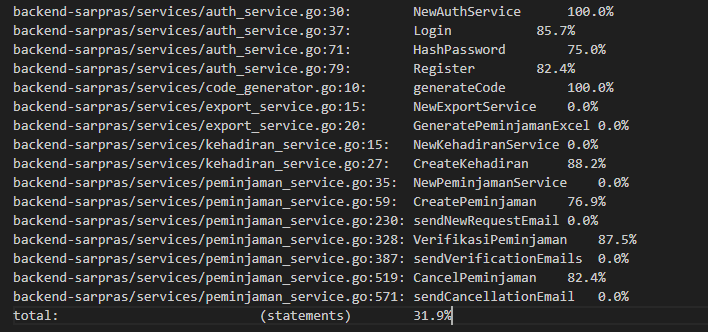
\includegraphics[width=0.9\textwidth]{gambar/media/image25.png}
    \caption{Ringkasan \textit{Code Coverage Backend}}
    \label{fig:coverage_summary}
\end{figure}

\subsection*{A.2 Detail \textit{Coverage}: \textit{Auth Service}}

Detail \textit{coverage} \textit{Auth Service} menunjukkan sebagian besar kode telah tercakup pengujian (hijau), termasuk fungsi kritis seperti \textit{login} dan \textit{register}.

\begin{figure}[H]
    \centering
    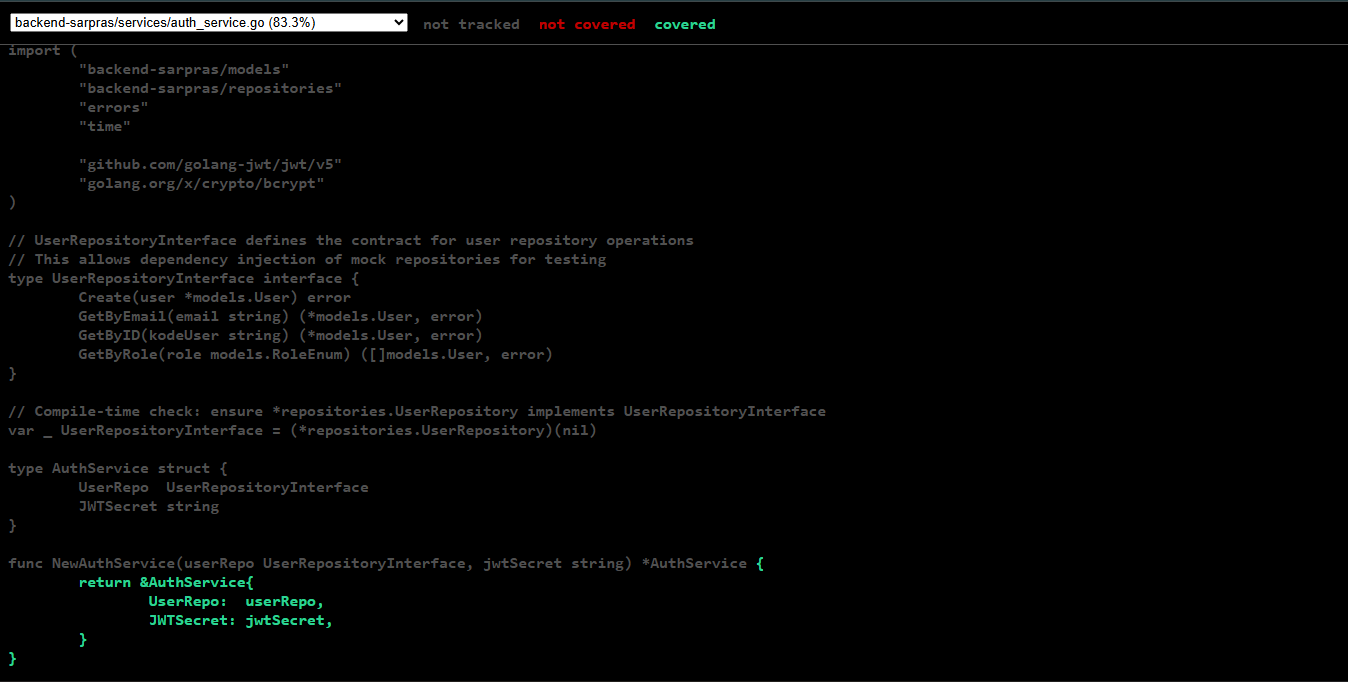
\includegraphics[width=0.9\textwidth]{gambar/media/auth service.png}
    \caption{Detail \textit{Coverage} \textit{Auth Service}}
    \label{fig:coverage_auth}
\end{figure}

\subsection*{A.3 Detail \textit{Coverage}: \textit{Kehadiran Service}}

Detail \textit{coverage} \textit{Kehadiran Service} menunjukkan tingkat \textit{coverage} tinggi (88,2\%), dengan fungsi utama \texttt{CreateKehadiran} telah diuji menyeluruh.

\begin{figure}[H]
    \centering
    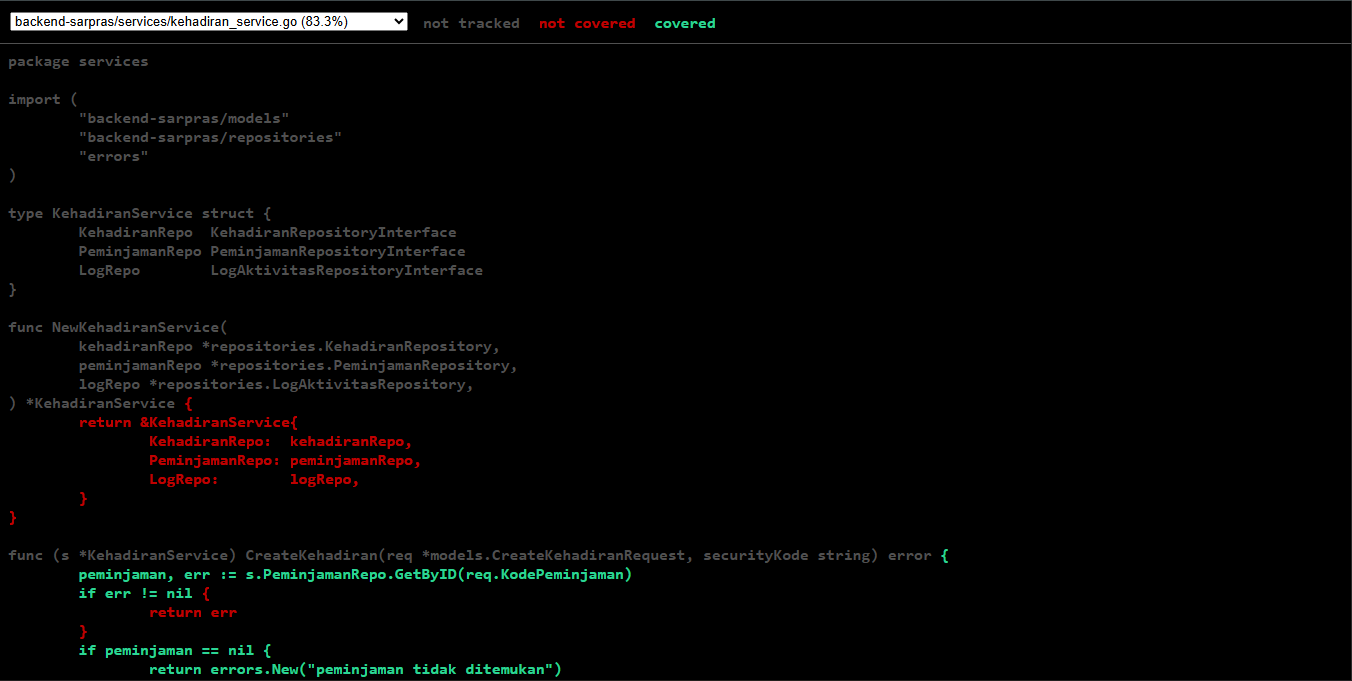
\includegraphics[width=0.9\textwidth]{gambar/media/kehadiran service.png}
    \caption{Detail \textit{Coverage} \textit{Kehadiran Service}}
    \label{fig:coverage_kehadiran}
\end{figure}

\subsection*{A.4 Detail \textit{Coverage}: \textit{Peminjaman Service}}

Detail \textit{coverage} \textit{Peminjaman Service} menunjukkan tingkat \textit{coverage} baik untuk fungsi inti (pengajuan, verifikasi, pembatalan peminjaman).

\begin{figure}[H]
    \centering
    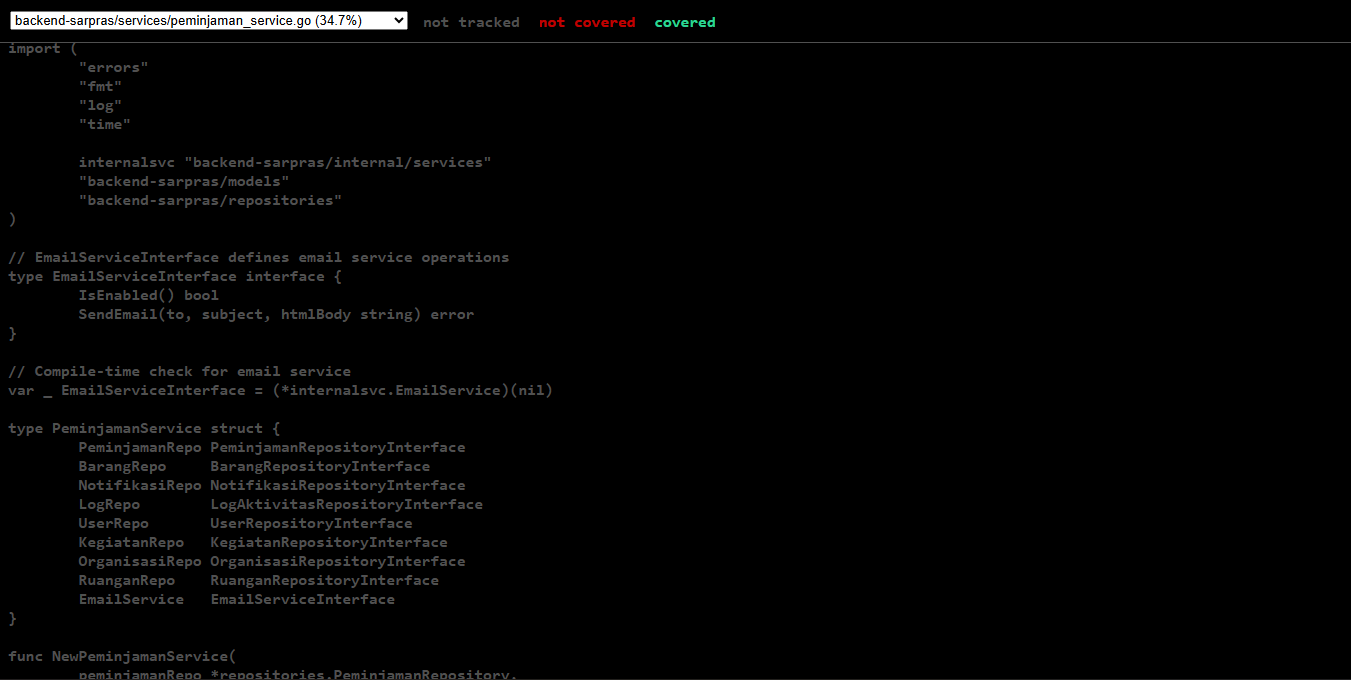
\includegraphics[width=0.9\textwidth]{gambar/media/peminjaman service.png}
    \caption{Detail \textit{Coverage} \textit{Peminjaman Service}}
    \label{fig:coverage_peminjaman}
\end{figure}

\section*{Lampiran B: Dokumentasi Wawancara}

Dokumentasi wawancara dengan staf Sarana dan Prasarana sebagai bagian proses pengumpulan data dan analisis kebutuhan sistem.

\begin{figure}[H]
    \centering
    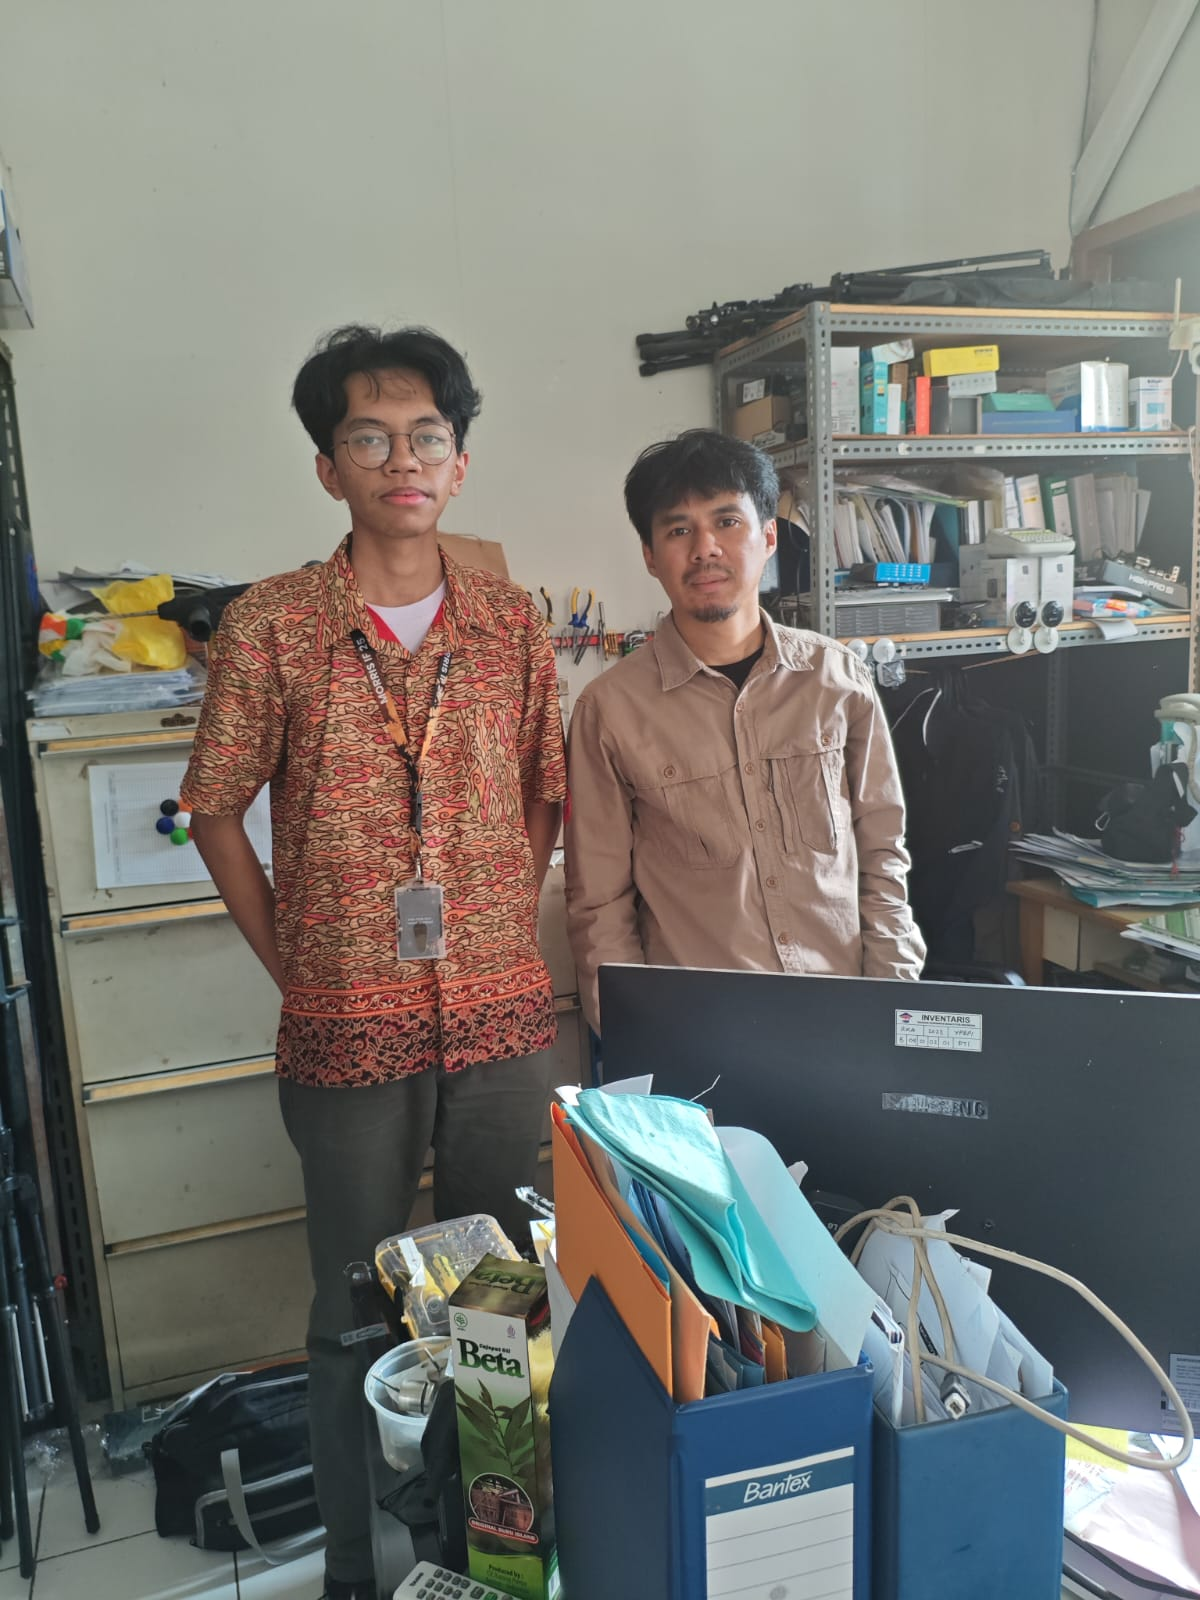
\includegraphics[width=0.5\textwidth]{gambar/media/coblong.jpeg}
    \caption{Dokumentasi Wawancara dengan Staf Sarana dan Prasarana}
    \label{fig:dokumentasi_wawancara}
\end{figure}


\clearpage

\end{document}
